%% IFBTcc Latex Template Version
%% 	based on a fork of : RiSE Latex Template
%%
%% IFBthesis latex template for thesis and dissertations
%% https://github.com/IFBmodels/tcc
%%
%% (c) 2017 Rafael de Campos Passos (rcpassos@ieee.org)
%%
%% This document was initially based on RiSE Latex template, from Yguaratã
%% Cerqueira Cavalcanti
%%
%% GENERAL INSTRUCTIONS
%%
%% We strongly recommend you to compile your documents using pdflatex command.
%% It is also recommend use the texlipse plugin for Eclipse to edit your documents.
%%
%% Options for \documentclass command:
%%         * Idiom
%%           pt   - Portguese (default)
%%           en   - English
%%
%%         * Text type
%%           bsc  - B.Sc. Thesis
%%           msc  - M.Sc. Thesis (default)
%%           qual - PHD qualification (not tested yet)
%%           prop - PHD proposal (not tested yet)
%%           phd  - PHD thesis
%%
%%         * Media
%%           scr  - to eletronic version (PDF) / see the users guide
%%
%%         * Pagination
%%           oneside - unique face press
%%           twoside - two faces press
%%
%%		   * Line spacing
%%           singlespacing  - the same as using \linespread{1}
%%           onehalfspacing - the same as using \linespread{1.3}
%%           doublespacing  - the same as using \linespread{1.6}
%%
%% Reference commands. Use the following commands to make references in your
%% text:
%%          \figref  -- for Figure reference
%%          \tabref  -- for Table reference
%%          \eqnref  -- for equation reference
%%          \chapref -- for chapter reference
%%          \secref  -- for section reference
%%          \appref  -- for appendix reference
%%          \axiref  -- for axiom reference
%%          \conjref -- for conjecture reference
%%          \defref  -- for definition reference
%%          \lemref  -- for lemma reference
%%          \theoref -- for theorem reference
%%          \corref  -- for corollary reference
%%          \propref -- for proprosition reference
%%          \pgref   -- for page reference
%%
%%          Example: See \chapref{chap:introduction}. It will produce
%%                   'See Chapter 1', in case of English language.
%%
%% Citation commands:
%%          \citet (from natbib) -- To cite a reference as part of the narrative
%%          \citep (from natbib) -- To cite a reference between parenthesis
%%          citationblock environment -- To produce direct citation blocks according to the ABNT

\documentclass[pt,oneside,onehalfspacing,bsc]{ifbclass/ifbclass}

  \usepackage{colortbl}
  \usepackage{color}
  \usepackage[table]{xcolor}
  \usepackage{microtype}
  \usepackage{bibentry}
  \usepackage{subfigure}
  \usepackage{multirow}
  \usepackage{rotating}
  \usepackage{booktabs}
  \usepackage{pdfpages}
  \usepackage{caption}
  \usepackage{lipsum}
  \usepackage{sectsty}
  \usepackage{tikz}
  \usepackage{amsmath}
  
  %% Set the language used in your code in the block above
  
  \captionsetup[table]{position=top,justification=centering,width=.85\textwidth,labelfont=bf,font=footnotesize}
  \captionsetup[lstlisting]{position=top,justification=centering,width=.85\textwidth,labelfont=bf,font=footnotesize}
  \captionsetup[figure]{position=bottom,justification=centering,width=.85\textwidth,labelfont=bf,font=footnotesize}
  
  %% Chapter and (Sub)Section fonts must be same size as text (12)
  \sectionfont{\fontsize{12}{15}\selectfont}
  \subsectionfont{\fontsize{12}{15}\selectfont}
  \subsubsectionfont{\fontsize{12}{15}\selectfont}
  
  %% Change the following pdf author attribute name to your name.
  \usepackage[linkcolor=black,
              citecolor=black,
              urlcolor=black,
              colorlinks,
              pdfpagelabels,
              pdftitle={IFB tcc Template (ABNT)},
              pdfauthor={ifb ctag team},
              breaklinks=true]{hyperref}
  
  \address{BRASÍLIA}
  
  \universitypt{Instituto Federal de Educação, Ciência e Tecnologia de Brasília, \textit{campus} Taguatinga,}
  \universityen{Federal Institute of Brasilia}
  
  \campus{Campus Taguatinga}
  
  \majorfieldpt{Bacharelado em Ciência da Computação}
  \majorfielden{Computer Science}
  
  \title{Extração de características em snoRNAs usando modelos matemáticos}
  
  \date{2022}
  
  \author{Marcos Bezerra Campos}
  \adviser{João Victor de Araújo Oliveira}
  
  % Macros (defines your own macros here, if needed)
  \def\x{\checkmark}
  %\let\lstlistoflistings\origlstoflistings
  \begin{document}

  \frontmatter
  \frontpage
  \presentationpage
  
  \begin{fichacatalografica}
    %\FakeFichaCatalografica % Comment this line when you have the correct file
  %     \includepdf{fig_ficha_catalografica.pdf} % Uncomment this
  \end{fichacatalografica}
  
  %\banca
  
  \begin{dedicatory}
  Dedico este trabalho à todas as pessoas que me incentivaram, apoiaram e forneceram todo o suporte necessário para a construção da tese.
  \end{dedicatory}
  
  \acknowledgements
  Agradeço à minha família por sempre ter me apoiado a estudar, principalmente aos meus pais que me nunca deixaram de prestar o suporte necessário durante a minha jornada. Ao Instituto Federal de Brasília (IFB) em conjunto com os docentes por terem consolidado o conhecimento necessário para chegar a esta etapa. Em especial ao orientador João Vitor, por ter me guiado e prestado assistência desde o início da realização do trabalho. E, claro, aos amigos e colegas que criei nessa jornada os quais convivi por longos anos e que me ajudaram a crescer em todos os aspectos. 
  
  \begin{epigraph}[]{Nelson Mandela}
  Não há paixão a ser encontrada apostando pequeno - em se contentar com uma vida que é menor do que aquela que você é capaz de viver.
  \end{epigraph}
  
  \resumo
  % Escreva seu resumo no arquivo resumo.tex
  {\parindent0pt
    O número de sequências biológicas disponíveis aumentou significativamente nos últimos anos devido a várias descobertas científicas sobre o código genético que compõe os seres vivos, criando um enorme volume de dados. Por consequência, novos métodos computacionais foram moldados para analisar e extrair informações dessas sequências genéticas. Os métodos de aprendizagem de máquina têm mostrado ampla aplicabilidade em bioinformática e demonstrou ser imprescendível para a extração de informações úteis das estruturas secundárias dos genomas ao aperfeiçoar suas técnicas com base no arquétipo matemático em contraste com o modelo padrão biológico de análise. No entanto, ainda existem vários problemas que motivam novas abordagens, principalmente envolvendo problemas de extração de características em estruturas extremamente pequenas como os snoRNAs. Considerando isso, o foco do trabalho é estudar e analisar os algoritmos de extração de características baseado em modelos matemáticos como o mapeamento numérico, a transformação de Fourier, entropia e redes complexas, tendo como estudo de caso as duas classes principais de snoRNAs: \textit{C/D box} e \textit{H/ACA box}. De forma concisa, definimos o estudo de caso em um pipeline dividido em ciclos fundamentado nas bases do \textit{machine learning} que guiará a pesquisa solidificando o comparativo entre o paradigma matemático adotado e os métodos biológicos casuais. 

\begin{keywords}
RNAs não codificadores, snoRNAs, Aprendizagem de Máquina, Modelos matemáticos de extração de características
\end{keywords}
  }
  
  \abstract
  % Write your abstract in a file called abstract.tex
  {\parindent0pt
    The number of available biological sequences has increased significantly in recent years due to several scientific discoveries about the genetic code stored in living organisms, creating a huge volume of data. Consequently, new computational methods were shaped to analyze and extract information from these genetic sequences. Machine learning methods have shown wide applicability in bioinformatics and proved invaluable for extracting useful information from the secondary structures of genomes by perfecting their techniques based on the mathematical archetype as opposed to the standard biological model of analysis. However, there are still several problems that motivate new approaches, mainly involving problems of feature extraction in extremely small structures such as snoRNAs. Considering this, the focus of the work is to study and analyze the feature extraction algorithms based on mathematical models such as numerical mapping, Fourier transformation, entropy and complex networks, having as a case study the two main classes of snoRNAs: \textit {C/D box} and \textit{H/ACA box}. Concisely, we define the case study in a pipeline divided into cycles based on the bases of \textit{machine learning} that will guide the research solidifying the comparison between the adopted mathematical paradigm and casual biological methods.

\begin{keywords}
non-coding RNAs, snoRNAs, Machine Learning, Mathematical Feature Extraction
\end{keywords}
  }
  
  % List of figures
  \listoffigures
  
  % List of Codes
  \lstlistoflistings
  
  % List of tables
  \listoftables
  
  % List of acronyms
  % Acronyms manual: http://linorg.usp.br/CTAN/macros/latex/contrib/acronym/acronym.pdf
  \listofacronyms
  \begin{acronym}[ACRONYM] 
% Change the word ACRONYM above to change the acronym column width.
% The column width is equals to the width of the word that you put.
% Read the manual about acronym package for more examples:
%   http://linorg.usp.br/CTAN/macros/latex/contrib/acronym/acronym.pdf
\acro{rnas}[RNAs]{Ácido ribonucleicos}
\acro{lncRNA}[lncRNAs]{Ácido ribonucleicos não-codificantes longos}
\acro{ncRNAs}[ncRNAs]{Ácido ribonucleicos não-codificantes}
\acro{ifb}[IFB]{Instituto Federal de Brasília}
\acro{unb}[UnB]{Universidade de Brasília}
\acro{question}[QP]{Questoes de pesquisa}
\acro{ci}[CI]{Critério de inclusão}
\acro{ce}[CE]{Critério de exclusão}
\acro{svm}[SVM]{Máquina de vetores de suporte}
\acro{ml}[ML]{Aprendizado de máquina}
\acro{glr}[GLR]{Generalized Linear Regression}
\acro{ga}[GA]{Algoritmo genético}
\acro{eden}[EDeN]{Explicit Decomposition with Neighborhoods}
\acro{nspdk}[NSPDK]{Neighborhood Subgraph Pairwise Distance Kernel}
\acro{cnn}[CNN]{Convolutional neural network}


\end{acronym}
  
  % Summary (tables of contents)
  \tableofcontents
  
  \mainmatter
  
  \chapter{Introdução}
\label{chp:introduction}

A expansão do Aprendizado de Máquina e de técnicas biológicas para a predição de estruturas protéicas e genômicas e também para o diagnóstico de doenças, trouxe um resultado significado no que tange a identificação de padrões e características em RNAs não-codificadores \textit{(ncRNAs)}. De acordo com \cite{math-feature-bio}, existem aplicações modernas que extraem propriedades biológicas relevantes para o estudo dessas moléculas como quadro de leitura aberto (\textit{ORF}), o uso da frequência de trigêmeos de nucleotídeos adjacentes e a porcentagem de conteúdo \textit{GC}. A aplicabilidade de cunho biológico, apesar de expressivo, dificilmente tem reutilização ou adaptação para problemas específicos tal como classificar as classes de RNAs não-codificadores.

Um exemplo disso é a classe de pequenos RNAs nucleolares \textit{snoRNAs} que podem ser divididos em duas classes: \textit{C/D box} e \textit{H/ACA box}. Em uma sequência \textit{ncRNA}, através da extração de características da estrutura secundária, em conjunto com técnicas de aprendizado supervisionado, auxiliam na identificação das classes \textit{C/D box} e \textit{H/ACA box} \textit{snoRNAs}, como visto na dissertação de \cite{snoRNAs-article}.

A construção de um modelo preditivo devido às limitações dos experimentos manuais no laboratório a fim de otimizar o desempenho dos modelos atuais de aprendizado de máquina também inclui uma representação matemática das sequências biológicas por meio do mapeamento numérico e a transformação de Fourier. A adoção de uma abordagem matemática no contexto de \textit{ncRNAs} demonstrou ser promissora nos experimentos de \cite{math-feature-bio} ao comparar a sua eficiência com os algoritmos particulamente de natureza biológica computacional. 

O pacote \textit{MathFeature}, proposto por \cite{math-features-package}, contém 37 \textit{features} descritivas para sequencias biologicas. Dentre estas 37, 20 são baseadas em uma analise matemática incluindo tanto a transformação de Fourier quanto o mapeamento numérico, mas também a entropia, grafos, redes complexas e CGR (\textit{Chaos game representation}) em sua composição. Os casos de estudo teve resultados experimentais significativos.

\section{Formulação do problema}

A extração de características busca gerar um vetor de características para uma determinada estrutura baseado no treinamento intensivo do modelo. A busca por técnicas de \textit{machine learning} capazes de identificar as características de estruturas secundárias de RNAs tornou-se fundamental ao longo dos últimos anos devido a grande quantidade de dados sobre o conteúdo genético. 

Os métodos casuais de extração de características do \textit{machine learning} nem sempre conseguem determinar um modelo eficaz que consiga evitar a perca de informações da estrutura, um bom exemplo disso é para as classes de pequenos nucleotídeos de RNA (snoRNAs). Para ilustrar a ideia, o estudo de \cite{math-feature-bio}, é relatado que a ténica \textit{ORF}, cuja é bastante aplicada no meio biológico para leitura sequencial do códon, retornou uma pontuação inferior a 0,009 para classificar o RNA circular de outros tipos de lncRNAs.

Além desse fato, os autores de \cite{math-features-package} mostraram que a eficiência de algoritmos para classificação de classes de lncRNAs demonstraram amplo provetio nos estudos de caso obtendo um desempenho entre 0.6350–0.9897 de eficácia na fase de avaliação, o que é extremamente vantajoso para a classificação de lncRNAs.

Diante disso, a questão norteadora do trabalho é assumida na hipótese a seguir:

\begin{itemize}
    \item \textbf{Hipótese} - Os métodos matemáticos, apesar de generalistas, são bons o suficiente como os biológicos para classificar as duas classes de snoRNAs: \textit{H/ACA box} e \textit{C/D box}.  
\end{itemize}

Pretende-se analisar e fundamentalizar a hipótese baseado nos resultados obtidos de experimentos em casos de testes. 

\section{Objetivos}
\subsection{Objetivos gerais}
    Este trabalho tem como objetivo geral a análise de modelos matemáticos de extração de características para as classes de snoRNAs.
    
\subsection{Objetivos específicos}

\begin{enumerate}
    \item Implementar um algoritmo de extração de \textit{features} com abordagem matemática como a transformação de Fourier, mapeamento numérico, entropia, redes convolucionais neurais, EDeN e etc;
    \item Extrair novas features de ambas as classes de snoRNAs (H/ACA box snoRNA e C/D box snoRNA);
    \item Validar o método matemático de aplicação generalista nas duas classes de snoRNAs;
    \item Comparar os resultados com os outros métodos de aprendizado de máquina, sejam eles híbridos ou biológicos;
\end{enumerate}
  \chapter{Referencial teórico}

\section{Bioinformática}

A bioinformática é a área de pesquisa que mescla as ciências biológicas e computacionais para o gerenciamento computacional de todos os tipos de informações biológicas moleculares, lidando com a estrutura e os aspectos funcionais dos genes e proteínas. Têm como objetivo desenvolver técnicas modernas para identificação de características do objeto de análise com o intuito de expandir a produção de farmacológicos, o descobrimento de vacinas, cura para doenças e vírus. Os estudos sobre o sequenciamento de moléculas genéticas e a análise sistemática de cadeias protéicas dos acidos nucleicos (DNAs e RNAs) evidenciaram que existe uma classe de pequenas moléculas de RNAs que desempenham um papel importante nos processos celulares. \cite{bio-info}

\subsection{Ácidos nucleicos}

De acordo com \cite{nucleic-acid}, ao que tange sobre ácidos nucleicos, são moléculas formadas por nucleotideos responsáveis por armazenar e transmitir as informações genéticas necessárias para a produção de proteínas, bem como a transcrição do conteúdo a partir do processo de reprodução celular. Os seres vivos, em sua composição, contém dois tipos importantes de ácidos nucleicos: o DNA e o RNA. O DNA (ácido desoxirribonucleico) detém a função de armazenar e transmitir essas informações enquanto o RNA (ácido ribonucleico) transcreve-as para formar a síntese protéica. 

Na biologia molecular, dois nucleotídeos em fitas complementares de DNA ou RNA que estão conectados por ligações de hidrogênio são chamados de par de bases nitrogenadas. No pareamento de bases Watson-Crick canônico no DNA, a adenina (A) forma um par de bases com a timina (T) usando duas ligações de hidrogênio, e a guanina (G) forma um par de bases com a citosina (C) usando três ligações de hidrogênio. No pareamento de bases Watson-Crick canônico no RNA, a timina é substituída por uracila (U). \cite{watson-crick-pair};

\begin{figure}[h]
    \centering
    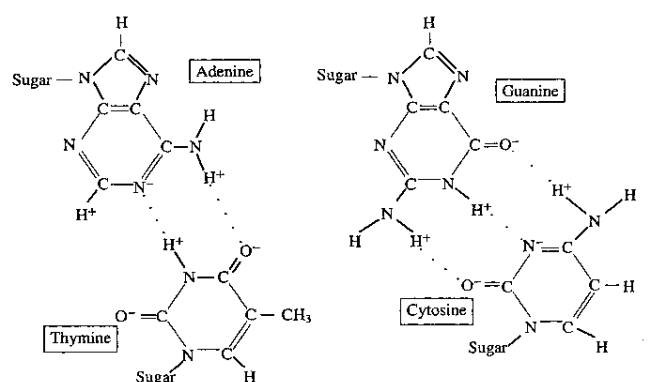
\includegraphics[width=0.7\textwidth]{images/pair-watson-crick.png}
    \caption{Extraído de \cite{nucleic-acid} para representar as ligações entre as bases nitrogenadas. }
    \label{fig:pair-watson-crick}
\end{figure}

\subsection{Mecanismo molecular e síntese protéica}

O mecanismo celular reconhece o início de um gene ou agrupamento de genes graças ao promotor, que
é uma região antes de cada gene no DNA que serve de indicação ao mecanismo celular que um gene está à frente. Tendo reconhecido o início de um gene ou agrupamento de genes, uma cópia do gene é feita em uma molécula de RNA. Este RNA resultante é o RNA mensageiro (\textit{mRNA}) e terá exatamente a mesma sequência que uma das fitas do gene, mas substituindo a base nitrogenada U por T. Esse processo é chamado de transcrição. O mRNA resultante será então usado em estruturas celulares chamadas ribossomos para fabricar uma proteína. 

Como o RNA é de fita simples e o DNA é de fita dupla, o mRNA produzido é idêntico em sequência a apenas uma das fitas gênicas, sendo complementar à outra fita - tendo em mente que T é substituído por U no RNA. A fita que se parece com o produto de mRNA é chamado de fita \textit{antisense} ou codificadora, e a outra é a fita \textit{sense} ou anticodificação ou então fita molde. A fita molde é a que realmente é transcrita, pois o mRNA é composto pela união de ribonucleotídeos complementares a esta fita.

A proteina é uma macromolécula formada por uma cadeia de aminoácidos pareadas por uma ligações peptídicas que conectam um átomo de carbono pertencente à carboxila a um ou mais átomos de nitrogênio. Ao efetuar a ligação, uma molécula de água é liberada porque o oxigênio e o hidrogênio da carboxila se une a um hidrogênio do grupo de amina. Assim, o que realmente encontramos dentro de uma cadeia polipeptídica é um resíduo do aminoácido original. As proteínas típicas contêm cerca de 300 resíduos, mas existem proteínas com apenas 100 ou com até 5.000 resíduos. \cite{nucleic-acid}
\\ \\ \\ \\ \\ \\ \\ 
\begin{figure}[h]
    \centering
    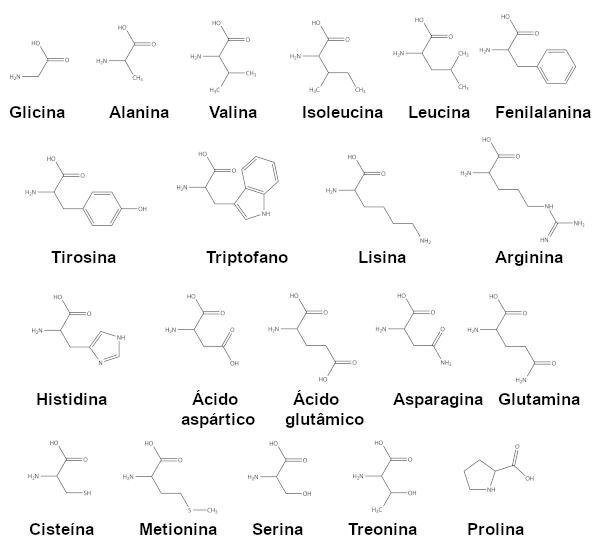
\includegraphics[width=0.65\textwidth]{images/aminoacidos.jpg}
    \caption{Moléculas de aminoácidos conhecidas.}
    \label{fig:aminoacidos}
\end{figure}

Portanto, para "especificar" uma proteína, é necessário decodificar cada aminoácido que ela contém. E isso é precisamente o que o DNA em um gene faz, usando triplas de nucleotídeos para especificar cada aminoácido. Cada tripla de nucleotídeos é chamado de códon. As triplas de nucleotídeos são dados usando bases de RNA em vez de bases de DNA, a razão é que são as moléculas de RNA que fornecem a ligação entre o DNA e a síntese protéica em um processo chamado de tradução. A conexão que designa a síntese protéica é feita entre um códon e o aminoácido que este códon codifica. Cada molécula de tRNA possui, de um lado, uma conformação que possui alta afinidade por um códon específico e, do outro lado, uma conformação que liga-se facilmente ao aminoácido correspondente. À medida que o RNA mensageiro passa o interior do ribossomo, um tRNA correspondente ao códon atual se liga a ele, trazendo o aminoácido. \cite{bio-info}

Um aspecto do processo de transcrição importante é o conceito de frame da leitura. Um quadro de leitura aberto, ou ORF, em uma sequência de DNA é um trecho contíguo dessa sequência começando no códon inicial, tendo um número inteiro de códons (seu comprimento é um múltiplo de três) tal que nenhum de seus códons seja um codão de terminação (uma tripla de nucleótidos que sinaliza a terminação da tradução). Uma das três formas possíveis de agrupar bases para formam códons em uma sequência de DNA ou RNA. Por exemplo, a sequência \textbf{TAATCGAATGGGC} pode ser decodificada tomando como códons TAA, TCG, AAT, GGG, deixando de fora o último C. Outro quadro de leitura seria ignorar o primeiro T e obter os códons AAT, CGA, ATG, GGC. Ainda outro quadro de leitura produziria os códons ATC, GAA, TGG, deixando de fora duas bases no início (TA) e duas bases no final (GC).\cite{stop-codon}

\begin{figure}[h]
    \centering
    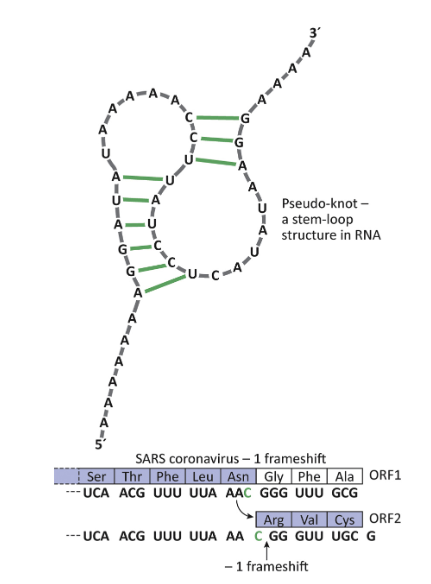
\includegraphics[width=0.65\textwidth]{images/covid_synthesis_proteic.png}
    \caption{Um pseudo-nó de RNA direcionando a estrutura ribossômica na síntese protéica. Extraído de \cite{stop-codon}}
    \label{fig:aminoacidos}
\end{figure}

\subsection{ncRNAs}

As regiões de proteínas não-codificadas abrangem 2\% do genoma humano e caracterizam por ser uma região a qual os RNAs detectados não são codificados a partir da síntese protéica. Os RNAs não traduzidos em proteínas foram nomeados RNAs não-codificadores (ncRNA) e foram considerados, a princípio, como um ruído ou subprodutos do fluxo de informação genética do DNA à proteína. A falta de dados científcos atribuindo funções para a maioria das regiões não codificantes do genoma reforça a ideia de que essa maioria pode realmente ser descartável. No entanto, hoje, é conhecido que os ncRNAs estão envolvidos em várias atividades celulares, como silenciamento de genes, replicação, regulação da expressão gênica, transcrição, estabilidade cromossômica, estabilidade de proteínas, translocação e localização, modificação de RNA, processamento e estabilidade. \cite{ncRNAs-intro}.

A predição de estruturas  conservadas é um fator preponderante para descobrir e caracterizar assinaturas para uma família de RNA específica. Ao tratar sobre ncRNAs, a sua identificação está
estritamente ligada à sua estrutura terciária e, como a estrutura terciária é determinada pela estrutura secundária, esta última é usada como uma aproximação no estudo de funções em ncRNAs. Se a função de um único RNA ou de uma família não for conhecida, pode-se inferir comparando a estrutura de RNA (ou consenso no caso de uma família) com um banco de dados de assinaturas estruturais secundárias. A comparação estrutural pode também ser usada para detectar a ocorrência de diferentes estruturas estáveis para a mesma molécula (o que pode indicar uma possível mudança na estrutura secundária impactando diretamente na sua função) para prever e comparar as mutações em uma sequência de RNA. \cite{ncRNAs-mitochondrial}

\begin{figure}[h]
    \centering
    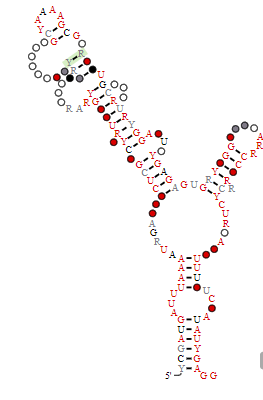
\includegraphics[width=0.5\textwidth]{images/secondary_structure_ncRNA.png}
    \caption{Estrutura secundária do icd-II ncRNA.}
    \label{fig:aminoacidos}
\end{figure}


A designação de famílias  de ncRNAs a partir da comparação estrutural secundária de sequências de ncRNAs, procurando RNAs homólogos a um candidato específico ou que pertence a uma família de candidatos continua sendo um problema específico da classificação de ncRNAs. Em tese, a pesquisa de ncRNA envolve três tipos principais de problemas de reconhecimento de padrões em ncRNas, segundo \cite{ncRNAs-content}, são eles:

\begin{itemize}
    \item Predição da estrutura secundária: O número de estruturas secundárias possíveis cresce exponencialmente com o comprimento da sequência. A questão é como buscar uma estrutura neste espaço de solução exponencial para escolher a melhor estrutura. Quando a estrutura secundária de apenas uma sequência de RNA precisa ser prevista, apenas métodos iniciais podem ser usado. Se um conjunto de RNAs homólogos estiver disponível, métodos comparativos podem prever a estrutura de consenso com mais precisão.
    
    \item Comparação de estrutura secundária: A comparação de estrutura calcula a diferença entre duas estruturas. A medição é feita calculando a diferença de uma distância de edição entre essas duas estruturas. A distância de edição depende de quantas operações de edição são necessárias para transformar uma das estruturas em outra considerando o custo de cada tipo de operação de edição. O cálculo da distância de edição está diretamente relacionada à forma como as estruturas são representadas e em que nível de resolução a comparação é realizada. Três maneiras comuns de representar estruturas são árvores, cadeias de colchetes e gráficos genéricos. Os níveis de resolução variam de pares de bases para padrões estruturais como hélices, loops e multi-loops.
    
    \item Identificação de RNA não codificadores: A detecção computacional direcionados a famílias de ncRNAs usam o máximo possível de peculiaridades. A criação de programas mais gerais que possam ser treinados para identificar características de uma família específica ou mesmo de uma única sequência de entrada é um caminho possível para identificação de famílias. Ainda assim, é desejável procurar novas famílias de genes, o que torna um problema para os programas de classificação geral de famílias conhecidas.
    
\end{itemize}

\subsection{snoRNAs}

Pequenos RNAs nucleolares (snoRNAs) são uma das mais antigas e numerosas famílias de RNAs não codificantes (ncRNAs), estão amplamente presentes nos nucléolos das células eucarióticas e têm um cumprimento de 60–300 nt. A principal função dos snoRNAs é guiar a modificação de rRNA específica do local. Em contraste, sua organização genômica e estratégias de expressão são as mais variadas. Aparentemente, as unidades de codificação de snoRNA adotaram, no curso da evolução, todas as formas possíveis de serem transcritas, proporcionando assim um paradigma único de flexibilidade de expressão gênica. \cite{snoRNAs-paradigm}

Os snoRNAs são codificados principalmente por regiões intrônicas de genes codificadores de proteínas e não codificadores de proteínas. Normalmente, podem ser classificados em três grupos: H/ACA box, C/D box e RNAs cajal pequenos (scaRNAs). Para \cite{snoRNAs-content}, os dois primeiros tipos de snoRNAs participam do processamento de RNA ribossômico (rRNA) adicionando modificações de 2-O-metilação e pseudouridilatação às moléculas de rRNA, respectivamente. No entanto, um tipo de snoRNAs estão localizados em corpos de Cajal (CBs), eles são chamados scaRNAs. Eles também seguem a classificação C/D-H/ACA, mas alguns scaRNAs contêm estruturas C/D e H/ACA. \textit{C/D box} snoRNAs se ligam a quatro proteínas essenciais – Nop1p, Nop56p,
Nop58p e Snu13p — para gerar pequenas ribonucleoproteínas nucleolar (snoRNPs). Da mesma forma, os snoRNAs de caixa H/ACA formam snoRNPs funcionais ligando-se a Cbf5p, Gar1p, Nhp2p e Nop10p.

O comprimento dos snoRNAs da \textit{C/D box} eucariótica geralmente varia de 70 a 120 nt. Esses snoRNAs contêm duas sequências conservadas: a \textit{C box e a D box}. A \textit{C box} consiste nos nucleotídeos \textbf{RUGAUGA}, que estão localizados na extremidade 5' da molécula de snoRNA. Em contraste, a \textit{D box} está localizada na extremidade 3' e consiste nos nucleotídeos \textbf{CUGA}. Juntos, esses elementos dependem do par de bases para dobrar em uma estrutura chamada \textit{kink-turn}. Essa estrutura é reconhecida pelo Snu13p, que então recruta Nop1p (também chamado fibrilarina [FBL]), Nop58p e Nop56p para modificação de 2'-O-metilação. \cite{snoRNAs-paradigm}.

\begin{figure}[h]
    \centering
    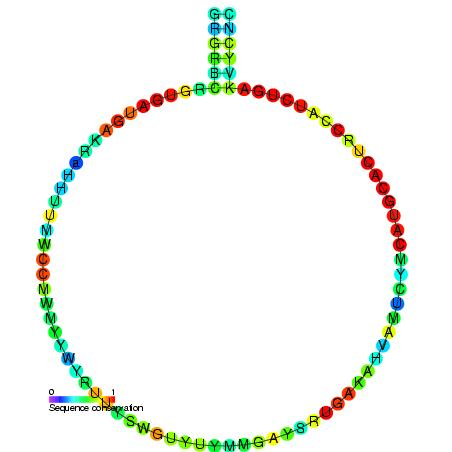
\includegraphics[width=0.5\textwidth]{images/snoRNA_c_d_box.jpg}
    \caption{Estrutura secundária do SNORD33, que pertence ao grupo \textit{C/D box}.}
    \label{fig:aminoacidos}
\end{figure}

Os snoRNAs \textit{H/ACA} geralmente têm 10 a 14 nt de comprimento e contêm a região chamada de bolsas de pseudouridilatação em que há resíduos de uridina no substrato RNA isomerizados. \textit{H/ACA box} snoRNPs se ligam a Cbf5p, Nop10p, Gar1p e Nhp2p, entre os quais
Cbf5p atua como a proteína catalítica envolvida na pseudouridilatação. Os snoRNAs eucarióticos H/ACA box contêm duas sequências: a \textit{H box} e a \textit{ACA box}, localizadas abaixo do primeiro e segundo \textit{hairpin}, respectivamente. \cite{snoRNAs-paradigm}.

\begin{figure}[h]
    \centering
    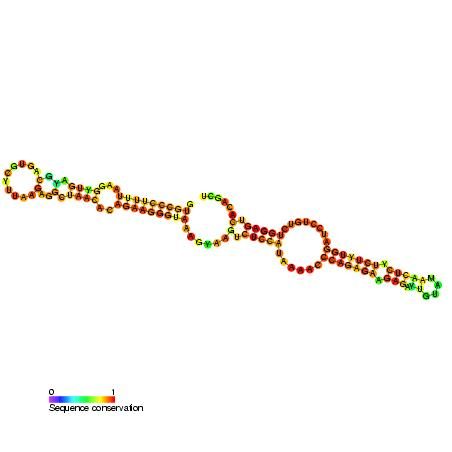
\includegraphics[width=0.5\textwidth]{images/snoRNA_h_aca_box.jpg}
    \caption{Estrutura secundária do SNORA26, que pertence ao grupo \textit{H/ACA box}.}
    \label{fig:aminoacidos}
\end{figure}


\section{\textit{Machine learning}}

De acordo com \cite{ml-approach}, o \ac{ml} é um ramo da inteligência artificial que envolve a autoaprendizagem do computador para executar tarefas. A seleção de características no aprendizado de máquina têm um papel significativo no desempenho dos modelos de previsão. É durante a seleção que a redundância e ruídos são identificados, a remoção do sobre-ajuste é aplicado, o que implica diretamente no aumento da velocidade de cálculo. Esta etapa crucial é capaz de definir as características discriminantes do objeto de estudo analisado.  Para entender melhor, o autor Mitchell, em \cite{ml-book}, explica o funcionamento do aprendizado de máquina sugerindo uma esquematização de um programa de computador o qual aprende a partir de uma experiência E através de alguma classe de tarefas T e uma medida de desempenho P. Vale ressaltar que sua performance para a tarefa T, medida em P, é aprimorada com a experiência E. Por exemplo, considerando a aplicabilidade do objeto de estudo da tese, considere que um programa deve classificar uma determinada sequência de código genético e precisa classificá-lo como um RNA, portanto:

\textbf{O problema pode ser traduzido para:}
\begin{itemize}
    \item Tarefa \textit{T}: Classificar o código genético em DNA ou RNA
    \item Medida de desempenho \textit{P}: Percentual de sequências de RNAs classificadas corretamente
    \item Experiência \textit{E}: Um banco de dados de sequências conhecidas de DNAs e de
sequências de RNAs
\end{itemize}

Dado um conjunto de dados, o algoritmo fará o treinamento a partir das características (\textit{features}) predefinidas que descrevem o RNA. A hipótese inicial é que haja uma função \textit{f} que consiga ser aplicável à um grupo \textit{X} de código genético que o caracterize como um RNA. O algoritmo não retorna uma solução exata, logo, a correlação do resultado é baseado na margem de erro da função heurística. Todavia, a intenção do aprendizado de máquina é que torne a máquina consistente ao armazenar a "experiência" ou informação advindas do banco de dados; quanto mais características estiver disponível para definir o caso de estudo, melhor. A determinação da acurácia é feita pelo valor resultante do \textit{F-score}, em termos estatísticos, é a medida de precisão de um teste, portanto, a escolha do conjunto de dados bem como a preferência do algoritmo impactam diretamente na sua eficácia. \cite{ml-intro}


\begin{figure}[h]
    \centering
    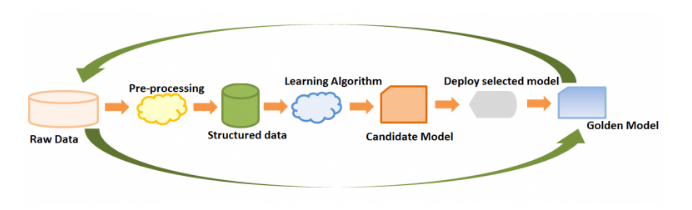
\includegraphics[width=0.8\textwidth]{images/workflow.png}
    \caption{Fluxo de trabalho do aprendizado de máquina.}
    \label{fig:workflow}
\end{figure}

A figura ~\ref{fig:workflow} mostra um simples fluxo de trabalho do aprendizado de máquina, inclusive, muito utilizado na mineração de dados: na primeira etapa recebe o dado bruto e em seguida passa para a etapa de pré-processamento que filtrará os dados e os limpará deixando-o estruturado, em sequência o algoritmo escolhido é executado e retornará o "modelo de candidado" para o treinamento em questão, a verificação do F-score é feito na fase seguinte e o "modelo de ouro", isto é, o grupo classificado que obteve a maior acurácia é encontrado. \cite{ml-intro}
O aprendizado de máquina é dividido em três grupos: aprendizado supervisionado, não supervisionado e reforçado. O aprendizado híbrido, por sua vez, combina ambos métodos: supervisionado e não supervisionado.

No estudo de \cite{ml-intro}, define-se que o aprendizado supervisionado mapeia uma entrada para uma saída com base em um conjunto de dados conhecidos, a saída é uma classe (no caso de classificação) ou um valor (em regressão linear). Na aprendizagem não supervisionada, os algoritmos construem modelos capazes de descrever os dados e as relações encontradas sem o uso de rótulos, além de incluir a divisão de dados em grupos (no caso de agrupamento) e resume a distribuição de dados em densidade estimativa. A aprendizagem por reforço envolve ações de aprendizagem em vez de classe, e a entrada é mapeada para ações com base no retorno, logo, é orientada a ação, onde são mantidas as ações que conterem maior recompensa. Para elucidar, as próximas seções abordarão alguns algoritmos de classificação importantes como \textit{SVM}, \textit{CNN} e \textit{Explicit Decomposition with Neighborhoods} (EDeN) para ilustrar alguns dos métodos disponíveis do aprendizado de máquina.

\subsection{SVM}

O SVM é um método não paramétrico que não é limitado pelo tamanho do conjunto de dados de treinamento. Essencialmente, o SVM gera modelos usados para classificação e regressão \cite{svm-1}. Em ambos os casos, se o SVM não for capaz de criar os vetores de suporte, ele pode construir hiperplanos em uma dimensão alta no espaço euclidiano para que ele selecione aqueles com maior margem, relacionados aos dados de treinamento \cite{svm-content}.  Nessas circunstâncias, o modelo SVM tenta encontrar uma reta para distinguir os grupos da entrada do conjunto de dados, excluso os casos em que as margens não podem ser criadas quando métodos simples de separação linear são usados para dados não-lineares. 

Com a finalidade de resolver este obstáculo, o SVM usa funções do kernel para aumentar a dimensão do espaço, de modo que o conjunto de dados possa ser linearmente separável em dimensões mais altas.

\begin{figure}[h]
    \centering
    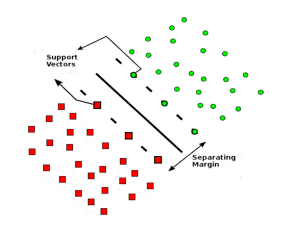
\includegraphics[width=0.5\textwidth]{images/svm_1.png}
    \caption{Exemplo de vetores de suporte de 2 dimensões adaptado por \cite{svm-content}.}
    \label{fig:svm_1}
\end{figure}

\begin{figure}[h]
    \centering
    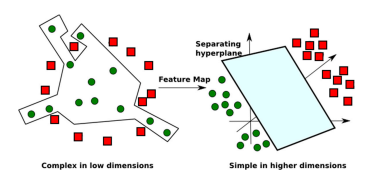
\includegraphics[width=0.5\textwidth]{images/svm_2.png}
    \caption{Dados separáveis não lineares em baixa dimensão, mapeados para uma dimensão mais alta; adaptado por \cite{svm-content}.}
    \label{fig:svm_2}
\end{figure}

Uma noção que é central para a construção do algoritmo de aprendizado do vetor de suporte é o kernel do produto interno entre um "vetor de suporte" xi e o vetor x extraído do espaço de entrada. Os vetores de suporte consistem em um pequeno subconjunto dos dados de treinamento extraídos pelo algoritmo

\subsection{\textit{CNN}}

O trabalho de Hubel e Wiesel em 1962 sobre a descoberta de atividades 
elétricas de neurônios em gatos foi pioneira para o desenvolvimento do método de aprendizagem de máquina baseada em multicamadas de neurônios, chamada de rede convolucional neural (CNN) \cite{hubel-wiesel}.Uma rede convolucional é um perceptron multicamada projetado especificamente para reconhecer formas bidimensionais com um alto grau de invariância à tradução, dimensionamento e distorção. Esta tarefa é aprendida de forma supervisionada por meio da rede cuja estrutura inclui as seguintes formas de restrições \cite{svm-content}:

\begin{enumerate}
    \item Extração de características - Cada neurônio recebe suas entradas sinápticas de um campo receptivo local na camada anterior, forçando-o a extrair características locais. Uma vez que um recurso foi extraído, sua localização exata torna-se menos importante, desde que sua posição em relação a outras características seja aproximadamente preservada.
    \item Mapeamento de extrações - Cada camada computacional da rede é composta de vários mapas de características, com cada mapa de características na forma de um plano dentro do qual os neurônios individuais são restringidos a compartilhar o mesmo conjunto de pesos sinápticos. Esta segunda forma de restrição estrutural tem efeitos benéficos como a invariância de deslocamento e redução da quantidade de parâmetros livres recebidos pelos perceptrons.
    \item Subamostragem - Cada camada convolucional é seguida por uma camada computacional que realiza média local e subamostragem, reduzindo a resolução do mapa de características. Esta operação tem o efeito de reduzir a sensibilidade da saída do mapa de características para deslocamentos e outras formas de distorção.
\end{enumerate}

\begin{figure}[h]
    \centering
    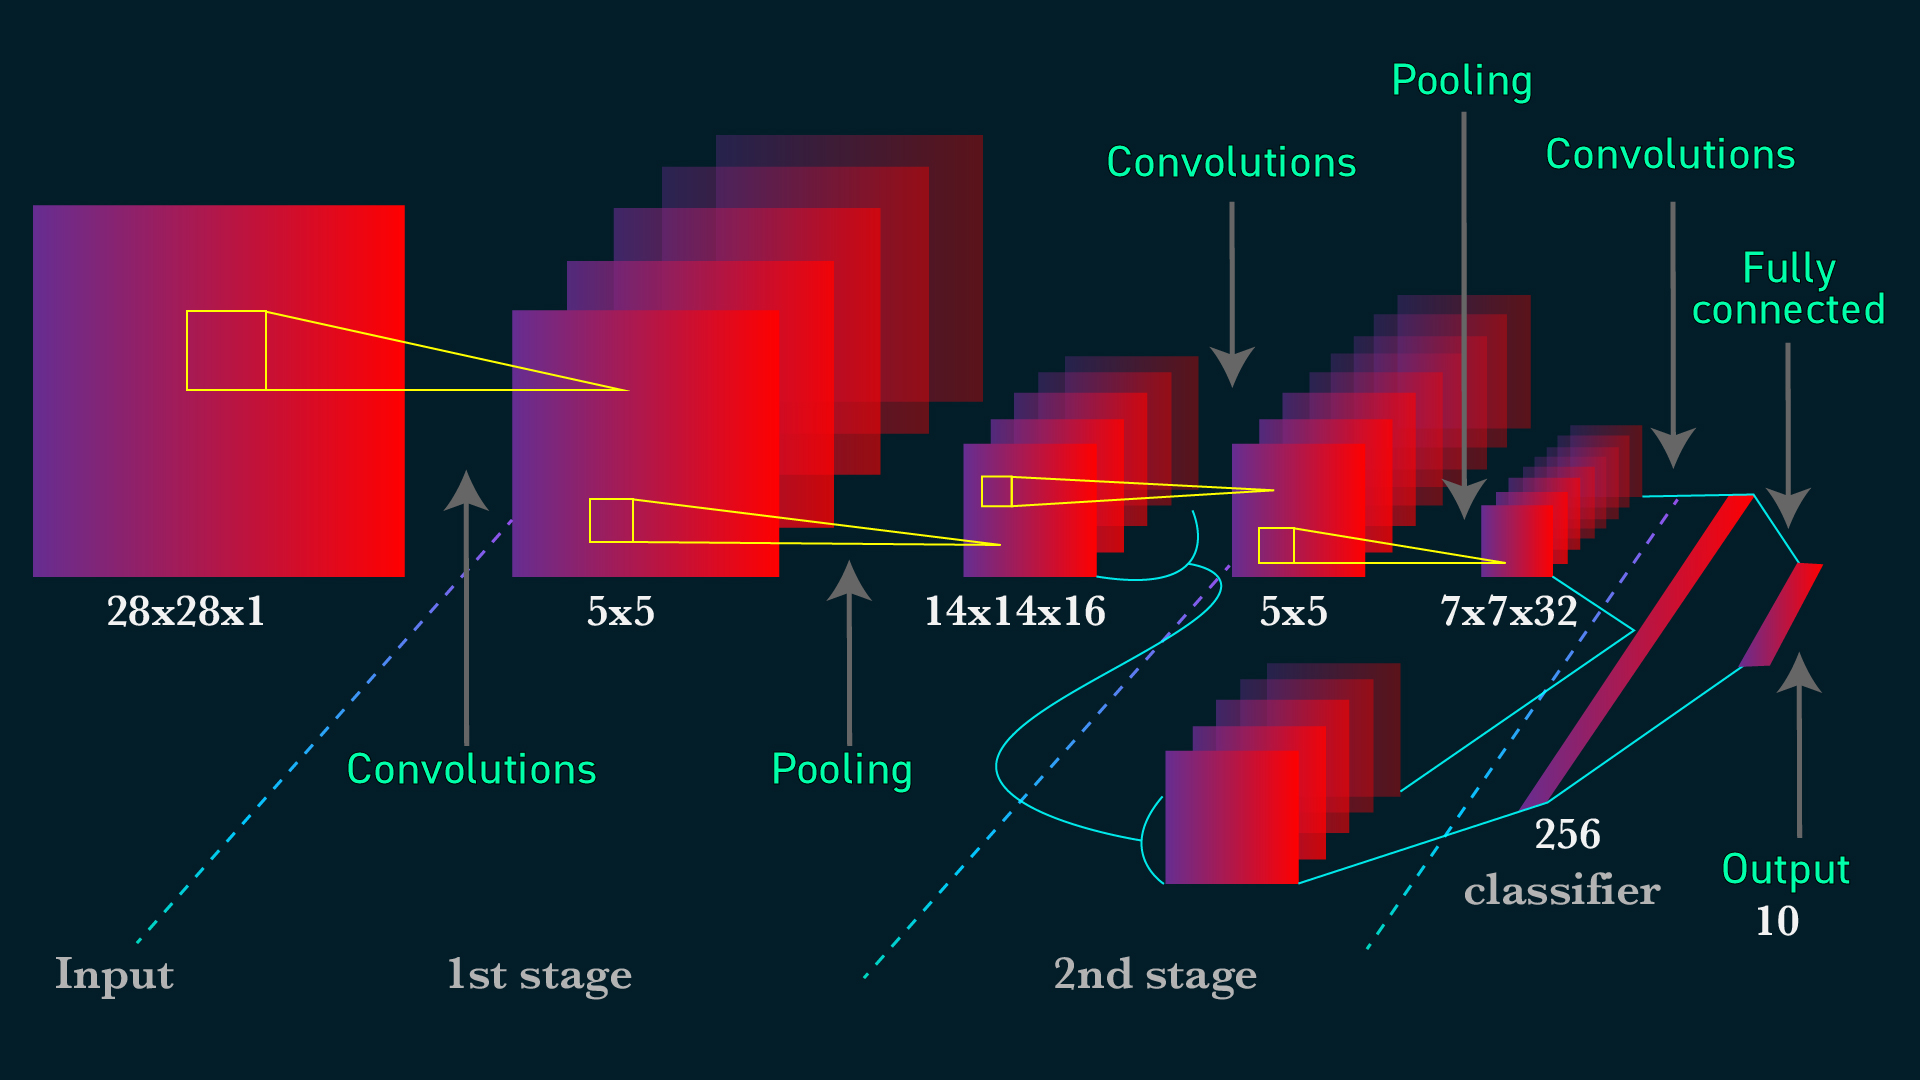
\includegraphics[width=0.55\textwidth]{images/cnn.jpg}
    \caption{Representação da rede convolucional neural no processamento de imagens (I) entrada de dados, (II) primeiro estágio, (III) segundo estágio, (IV) classificador de 256 pixels, (V) saída com 10 pixels totalmente conectada; Imagem extraída de \cite{cnn-image}.}
    \label{fig:cnn}
\end{figure}

A essência da rede neural convolucional é baseada na retropropagação que consiste na atualização contínua dos pesos para que os neurônios com a maior taxa de erro/perca sejam minimizados garantindo a consistência do modelo e a acurácia do método. A retropropagação funciona da seguinte forma: ao adentrarmos ao mapeamento de extrações, é necessário atualizar o peso de cada sináptico (ligação entre dois neurônios) de forma que aplique em todos os neurônios das camadas anteriores e para que isso seja implementado, é necessário a função de perca e a de hipótese, elas guiarão o modelo pela a rede inteira até que chegamos a uma camada final que seja utilizável \cite{cnn-blog}.

Portanto, conforme o mapeamento de extrações avança, os pesos tendem a diminuir pois são cálculos a partir da derivada parcial das funções. Consequentemente, o último nó da rede armazenará o total de perda do modelo que será usado para a avaliação do resultado, percebe-se, então, que a rede convolucional vai aprendendo a classificar o modelo por treinamento extraindo suas próprias características esporadicamente.

\subsection{EDeN}

\textit{Explicit Decomposition with Neighborhoods} (EDeN) é um kernel decomposicional de grafos baseado no \textit{Neighborhood Subgraph Pairwise Distance Kernel} (NSPDK) que produz um subgrafo da estrutura secundária do snoRNAs e produz um conjunto explícito de \textit{features} usado para algoritmos de aprendizagem de máquina supervisionados, não-supervisionados ou híbridos de maneira escalável.

A decomposição de uma sequência genômica em partes de objeto pretende conceber um kernel local válido entre as subpartes para que seja obtido uma função de similaridade capaz de decompor exponencialmente se existir um método que enumere os kernels em tempo polinomial recorrendo a programação dinâmica para tal ato. À medida que a dimensão do espaço de características torna-se maior, há uma probabilidade de que uma fração das dimensões não serão correlacionadas com a função de similaridade. Como consequência, mesmo usando algoritmos de classificação com margem alta, tornam-se obsoletos para determinar uma boa generalização do modelo. \cite{eden-nspdk}

\begin{figure}[h]
    \centering
    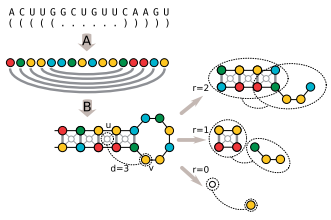
\includegraphics[width=0.6\textwidth]{images/eden_graph.png}
    \caption{\textbf{Codificação da estrutura secundária de RNA e as \textit{features} do kernel do grafo}; Imagem extraída de \cite{graph-representation}.}
    \label{fig:eden_graph}
\end{figure}

Para entender melhor como funciona a tradução da sequência para um grafo, o passo-a-passo da codificação da estrutura secundária é: \textbf{(A)} A codificação do grafo preserva a informação do nucleotídeo (rótulos do vértice) e os pares de bases (rótulos da borda), aqui representados com cores diferentes. \textbf{(B)} Vértices adicionais são inseridos para induzir \textit{features} relacionados ao empilhamento quádruplo de pares de base (vértices finos de cor cinza no centro de cada empilhamento de pares). Na parte da direita exemplo de \textit{features} induzidas pelo kernel do grafo \textit{NSPDK} para um par de vértices \textbf{u,v} na distância 3 com raio 0,1,2. Os grafos de vizinhança são encerrados em trilhas tracejadas.

Em uma conotação matemática, proposto por \cite{graph-representation}, dado um grafo $G = (V,E)$, em que $V$ é o conjunto de vértices e o $E$ é o conjunto de arestas. Sendo a distância de dois vértices $u,v$ denotada por $D(u, v)$ do menor caminho entre eles e o raio $r$ da região do subgrafo induzido é o conjunto de vértices a uma distância $d$ menor ou igual a $r$ de $v$. Considere que $N_{v,r}$ (G) denota o subgrafo de vizinhança, ou seja, o subgrafo de $G$ enraizado em $v$ induzido pelo conjunto de vértices. A relação de pares de vizinhança $R_{r,d}$ é definida como válida quando a distância entre as raízes de dois subgrafos de vizinhança de raio $r$ é exatamente igual a d. O kernel de decomposição, portanto, $k_{r,d}$ na relação $R_{r,d}$ em um NSPDK pode ser definido da seguinte forma: 

\begin{equation}
    K(G, G^{'}) = \sum_{r}^{r^{*}} \sum_{d}^{d^{*}}k_{r,d}(G, G^{'})
\end{equation}

Isto significa que o NSPDK decompõe o grafo em pares de subgrafos
vizinhos limitando a soma de $k_{r,d}$ kernels a cada iteração para todos os valores crescentes do parâmetro de raio $r$ e distância $d$ até um valor máximo dado $r^{*}$ e $d^{*}$ respectivamente.
  \chapter{Revisão da literatura}

A construção do estado de conhecimento teve como princípio a análise sistemática de dissertações, teses, trabalhos científicos e artigos produzidos em um lapso temporal de 6 anos. A estratégia utilizada para a revisão sistemática da literatura busca seguir os critérios adotados por \cite{review-literature} tendo o trabalho de \cite{math-feature-bio} como exemplo.

\section{Questões de pesquisa}
As questões de pesquisa norteam a revisão sistemática e têm como objetivo definir a parametrização da problemática identificando os trabalhos que propunham a extração de características em sequências de RNAs, quais métodos de extração matemáticos bem como o comparativo da técnica biológica em detrimento dos modelos matemáticos e a acurácia de cada método considerando um grupo de lcRNAs. Portanto, as \ac{question} foram definidas a seguir:

\begin{itemize}
   \item\ac{question}$_{1}$ Quais os métodos de extração de características em sequências de RNAs?
  \item \ac{question}$_{2}$ Quais os modelos matemáticos utilizados na extração?
  \item \ac{question}$_{3}$ Quais os grupos de lcRNAs a serem trabalhados e os modelos matemáticos aplicados?
\end{itemize}

\section{Estratégia de busca}

As bases de dados \textit{PubMed Central}, repositório da UnB, \textit{Oxford Academic}, \textit{Medline}, SIABI/IFB foram consumidas para embasamento teórico e argumentativo da tese. O \textit{PubMed Central} é um banco de dados digital gratuito de literatura científica na área de biomedicina e tecnologia gerenciado e desenvolvido pela \textit{National Library of Medicine} que contém um vasto repositório de artigos científicos mundialmente reconhecido. O repositório da UnB é um serviço digital oferecido pela Biblioteca Central para a gestão e disseminação da produção científica da Universidade de Brasília. A base da \textit{Oxford Academic} publica os periódicos de cunho científico geral para o público em mais alta qualidade, dispondo de uma comunidade acadêmica da Universidade de Oxford. A Medline que é uma biblioteca virtual de medicina a qual detém os dados indexados por uma palavra-chave específica do sistema \textit{MeSH} e, por fim, o SIABI/IFB, biblioteca virtual do IFB que disponibiliza os recursos dos campus existentes em Brasília.

\begin{table}[h!]
  \begin{center}
    \caption{Base de dados consumidas}
    \label{tab:table1}
    \begin{tabular}{l r} % <-- Alignments: 1st column left, 2nd middle and 3rd right, with vertical lines in between
      \hline \\
      \textbf{Base de dados} & \textbf{Link para acesso} \\ \\
      \hline \\
      \textbf{PubMed Central} & <https://pubmed.ncbi.nlm.nih.gov/> \\
      \textbf{Repositório UnB} & <https://repositorio.unb.br/> \\
      \textbf{Oxford Academic} & <https://academic.oup.com/journals>\\
      \textbf{Medline} & <http://bases.bireme.br/>\\
      \textbf{SIABI/IFB} & <http://siabi.ifb.edu.br/> 
      \\ \hline 
    \end{tabular}
  \end{center}
\end{table}

Para cada base de dados escolhida foram realizadas buscas avançadas em suas
ferramentas de pesquisa com um intervalo de tempo de 6 anos até a data de
realização desta revisão (24 de junho de 2022), contemplando como palavras-chaves de pesquisa: \textit{ncRNAs}, \textit{machine learning}, \textit{feature extraction}, \textit{sequence features}, \textit{mathematical approach} às quais resultaram em um conjunto de mais de 300 literaturas. Visando diminuir o escopo das produções para a problemática em questão, modificou-se o critério de análise que apenas considerava o título e resumo dos materiais e passou-se a levar em conta apenas os trabalhos que continham ncRNAs como objeto de estudo. Na seção posterior, mais especificamente no processo de seleção e exclusão, ao passar pela crítica qualitativa das obras, as literaturas serão menos abrangentes e mais voltadas ao estudo de caso da tese. A Tabela 3.2 mostra a quantidade de artigos científicos retornados por cada banco de dados no campo de busca.

\begin{table}[h!]
  \begin{center}
    \caption{Resultado das buscas nos bancos de dados}
    \label{tab:table2}
    \begin{tabular}{l c r} % <-- Alignments: 1st column left, 2nd middle and 3rd right, with vertical lines in between
      \hline \\
      \textbf{Base de dados} & \textbf{Palavras-chaves} & \textbf{Produções científicas} \\ \\
      \hline \\
      \textbf{PubMed Central} & \textit{Machine learning, sequence features, ncRNAs} & 98\\
      \textbf{Repositório UnB} & \textit{Machine learning, ncRNAs} & 5 \\
      \textbf{Oxford Academic} & \textit{Machine learning, ncRNAs, mathematic sequence features} & 153\\
      \textbf{Medline} & \textit{Machine learning, ncRNAs, mathematic sequence} & 34\\
      \textbf{SIABI/IFB} & \textit{Machine learning} & 2\\ 
      \hline \\
      \textbf{Total} & & 292  
    \end{tabular}
  \end{center}
\end{table}

\section{Critério de inclusão e exclusão}

Para responder as QPs definimos Critérios de Inclusão (CIs) e Critérios de Exclusão (CEs) que irão filtrar os resultados das pesquisas. Os CIs estão listados a seguir.

\begin{itemize}
  \item \ac{ci}$_{1}$ Produções científicas que usam os \ac{ncRNAs} como objeto de pesquisa para a extração de características;
  \item \ac{ci}$_{2}$ Estudos primários que aplicam modelos preditivos supervisionados ou não supervisionados sendo biológico, híbrido ou matemático para classificação de \ac{ncRNAs};
  \item \ac{ci}$_{3}$ Estudos que classificam as classes e grupos de ncRNAs aplicando o modelo matemático de extração de características;
\end{itemize}

Os \ac{ce} irão ajudar a filtrar apenas os artigos científicos relevantes para a revisão. Baseado nas questões de pesquisa que norteam o trabalho, os \ac{ce}s propostos abaixo selecionarão um grupo concreto de produções a fim de diminuir a abragência e a generalização do tema.

\begin{itemize}
    \item Estudos que não estejam escritos em português ou inglês;
    \item Estudos que a versão completa não é disponível gratuitamente;
    \item  Estudos "duplicados", que foram obtidos através da busca em mais de uma base, nestes casos apenas o primeiro será considerado.
    \item Produções científicas que não classificam o grupo de \ac{ncRNAs};
    \item Estudos descritivos de funcionalidades que não discorre sobre a metodologia de \ac{ml} empregue;
\end{itemize}


\section{Análise e discussão das literatuas}

As aplicações modernas do \textit{ML}  extraem informações relevantes de sequências baseadas em várias propriedades biológicas e físico-químicas, usando quadros de leitura abertos (ORF), frequência de uso de nucleotídeos adjacentes, conteúdo \textit{GC} e entre outros. Essas abordagens são comuns em problemas biológicos, mas essas implementações são muitas vezes difíceis de reutilizar ou adaptar a outro problema específico. Um grande exemplo é que os recursos ORF são um guia essencial para \ac{ncRNAs} de genes codificadores de proteínas, mas não são capazes de classificar classes para os ncRNAs, e, como dito por \cite{lncRNAs-article}, consequentemente, a extração de um conjunto de características que contêm informação discriminatória significativa para identificá-las é prejudicada, o que influencia na construção de um modelo preditivo. 


\cite{math-feature-bio} propõe um modelo preditivo matemático para identificação de classes de ncRNAs. Este trabalho foi dividido em três estudos de caso: (I) Avaliação das abordagens matemáticas com os problemas mais frequentes da classe de ncRNAs, por exemplo, \textit{lncRNA versus mRNA}; (II) Teste de generalização em diferentes classificadores de ncRNAs; (III) Análise de persistência em cenários com dados desbalanceados. As técnicas de \ac{ml} aplicadas consistem na transformação discreta de Fourier, mapeamento numérico (representação de Voss, de Real, de z-curve, de EIIP e de números complexos), entropia de Shannon e Tsallis e o uso de redes complexas. 

\cite{ga-svm} em contra-proposta aplica um \ac{ga} junto a uma \ac{svm} que implementa o método de aprendizado de máquina supervisionado baseado no conceito da teoria de Darwin, isto é, o conjunto de sequências que mais se adaptam a parametrização de classificação dos algoritmos são herdadas na próxima geração a partir do mecanismo de competição. Em suma, a classificação executa um modelo preditivo biológico na categorização do grupo de ncRNAs.

\cite{math-features-package} apresenta um pacote de 20 descritores matemáticos divididos em 5 grupos: mapeamento numérico, \textit{chaos game}, transformação de Fourier, entropia e grafos. Similar ao seu estudo comparativo \cite{math-feature-bio}, o autor executa o estudo de caso nos ncRNAs treinando o algoritmo \textit{CatBoost} para classificação de classes e concluiu que a abordagem matemática trouxe uma eficácia significativa nos resultados.

\cite{snoRNAs-article} busca classificar as classes de snoRNAs \textit{(H/ACA box snoRNA e C/D box snoRNA)} empregando uma técnica mais sofisticada na fase de treinamento no intuito de encontrar bons meta-parâmetros da \ac{svm}. A ideia é usar o \ac{eden}, um kernel decomposicional de grafos baseado no \ac{nspdk}, que pode ser usado para a geração explicita de features a partir de grafos e as \ac{svm}s que geram um hiperplano como superfície de decisão de tal modo que a margem de separação entre amostras positivas e negativas é maximizada formando, posteriormente, as classes preditas no hiperplano. 

\cite{snoReport-article} é a versão melhorada do snoReport 1.0, ferramenta cuja fora utilizada em \cite{snoRNAs-article} para a classificação de snoRNAs usando uma combinação de estruturas secundárias e \ac{ml}. A aprimoração do snoReport contemplou novos recursos para os snoRNAs \textit{box C/D e H/ACA box}, desenvolvendo uma técnica robusta na fase de treinamento da \ac{svm} (com dados recentes de organismos vertebrados e o refinamento dos parâmetros \textit{C} e \textit{gamma} na \ac{svm}), consumindo ainda mais bancos de dados para expandir a coleção anterior do snoReport. Para validar a sua serventia, houve diversos testes em organismos animais os quais mostraram um ótimo desempenho de classificação.

\cite{cnn-article} aborda a classificação de ncRNAs fundado nas redes neurais convolucionais. O treinamento é feito por representações distributivas de 4 nucleotídeos que derivaram com sucesso as matrizes de peso de posição em kernels aprendidos que correspondem a sequência de \textit{motifs} como locais de ligação a proteínas. A classificação de um par alinhado de duas sequências em classes positivas e negativas corresponde ao agrupamento das sequências de entrada. Depois de combinarmos a distribuição
representativa de nucleotídeos de RNA com a informação da estrutura secundária específica para \ac{ncRNAs}
e ainda com perfis de mapeamento de leituras de sequência de próxima geração, o treinamento de CNNs
para classificação de alinhamentos de sequências de RNA rendeu agrupamento preciso em termos de famílias ncRNA e superou os métodos de agrupamento existentes tradicionais para sequências de ncRNA. Interessantes sequências de \textit{motifs} e estruturas secundárias conhecidas pelas famílias de snoRNAs, microRNA e tRNAs foram identificadas no estudo.

\cite{graph-kernel-article} sugere um estudo voltado a classificação funcional de ncRNAs fundamentado na implementação de um grafo kernel. Para lidar com entidades representadas como grafos, uma variedade de
kernels têm sido propostos na literatura. Diferentes noções de similaridade são obtidas escolhendo diversos tipos de subestruturas a serem consideradas, desde caminhos até pequenos subgrafos. Existem várias maneiras de representar estruturas secundárias de RNA, incluindo as representações entre colchetes (onde os nucleotídeos são convertidos em nós e ligações em arestas) e representações em árvore (onde pares de bases são convertidos em nós 'tronco' e nucleotídeos de alça são convertidos em nós de 'loop'). Cada representaçãotem diferentes vantagens e desvantagens, incluindo perda de informações e complexidade
de cálculo. A estratégia \ac{nspdk}, assim como no trabalho de \cite{snoReport-article}, é adotada com o objetivo de materializar a codificação de características implícitas que é chave para obter eficiência linear na fase de classificação. Neste artigo, a representação escolhida é a \textit{loss-less}, ou seja, \textbf{sem perda}, onde os nós representam nucleotídeos e as arestas são as ligações entre eles, seja do tipo \textit{backbone} ou do tipo de \textit{encadernação}.

\cite{}

\section{Conclusão dos resultados apresentados na análise}

Através da análise e discussão dos resultados da revisão, percebemos que existe
a exploração de modelos preditivos matemáticos para a classificação de ncRNAs em oposição aos modelos tradicionais biológicos. Este fato deve-se pela alta taxa de \textit{F-score}, em outras palavras, da acurácia no classificamento de classes para os ncRNAs. Apesar da perspectiva biológica e híbrida, em contraste com a matemática, sua escolha varia de acordo com o objeto de estudo analisado e a sua eficiência de identificação. Há algoritmos que são melhores para classificação de móleculas de DNAs, assim como há outros mecanismos de classificação que produzem resultados significativos para as moléculas de RNAs. No atual contexto, os projetos científicos revelam que a extração de características por um cenário matemático demonstrou ser relevante para classificação de ncRNAs. O principal enfoque da tese é demonstrar o custo do algoritmo, o \textit{pipeline} das etapas a serem executadas desde a entrada, a parametrização, treinamento e testes até a saída. Mesmo que muito progresso já tenha sido feito, existem incógnitas para este grupo importante de moléculas que podem ser respondidas pelo avanço do \ac{ml}. Com base nas provas de conceito observadas é possível perceber a capacidade do modelo preditivo matemático de identificar os ncRNAs e do benefício da identificação em um âmbito biomedicinal.

% \section{Introduction}

% \lipsum[1]

% \begin{code}[language=Python,caption=Python Fribonacci Code,label=code:frib]
% from math import *

% # define function
% def analytic_fibonacci(n):
%   sqrt_5 = sqrt(5);
%   p = (1 + sqrt_5) / 2;
%   q = 1/p;
%   return int( (p**n + q**n) / sqrt_5 + 0.5 )

% for i in range(1,31):
%   print analytic_fibonacci(i)
% \end{code}


% This is a reference to Code \ref{code:frib} \ldots{}

% \lipsum[1]

% \begin{code}[language=C,caption=Hello World C Code,label=code:helloc]
% #include<stdio.h>

% main()
%     {
%         printf("Hello World");
%     }
% \end{code}


% This is a reference to Code \ref{code:helloc} \ldots{}

% \lipsum[1]

% \begin{code}[language=Java,caption=Hello Java Code,label=code:helloj]
% public class HelloWorld {

%     public static void main(String[] args) {
%         System.out.println("Hello, World");
%     }
% }
% \end{code}


% This is a reference to Code \ref{code:helloj} \ldots{}


% \section{Section}

% \lipsum[2-4]

% \subsection{Subsection}

% \lipsum[2-4]

  \chapter{Metodologia}


A metodologia está dividida nas seguintes etapas:

\subsection{Coleta de dados}

A busca por dados brutos das duas classes de snoRNAs será feita nos bancos de dados \textbf{RFAM}, \textbf{snorpy} e o snoDB. A coleta de dados agregará os snoRNAs encontrados em organismos vivos de plantas e humanos.

O \textbf{RFAM} \cite{rfam} é um banco de dados sobre snoRNAs que contém 792 famílias associadas a snoRNAs e possui cerca de 126.183 diferentes tipos de snoRNAs pertencentes a classe \textit{C/D box} e 34.368 tipos de snoRNAs da classe \textit{H/ACA box}.

O \textbf{snoPY} \cite{snoPY} é um banco de dados contém 6603 amostrar de snoRNAs da classe \textit{C/D box} com 41 espécies encontradas e 11176 amostrar de snoRNAs da classe \textit{H/ACA box} contendo 60 espécies informadas.

O \textbf{snoDB} \cite{snoDB} é um banco de dados especializado em snoRNAs extraídos de seres humanos hospedado por \textit{Scott Group Bioinformatics}, a sua versão 2.0, criada por Danny Bergeron, detém 510 amostras de snoRNAs da classe \textit{H/ACA box} e 1107 snoRNAs da classe \textit{C/D box}.

\subsection{Pré-processamento de dados}

A princípio, haverá dois conjuntos de dados: um contendo a classe \textit{H/ACA box} de snoRNAs com suas amostras positivas e negativas no conjunto e outro da classe \textit{C/D box}. A etapa de pré-processamento fará uma filtragem e limpeza no conjunto removendo a redundância, o sobreajuste, o subajuste e os valores atípicos. \cite{pre-process-ml}

\subsection{Extração de características}
A etapa de extração de características usará os algoritmos matemáticos para classificação de grupos como a transformação de Fourier, mapeamento numérico (inteiro, real, etc), SVM (máquina de suporte de vetores), SVD (decomposição singular de valores), entropia e CNN (rede neural convolucional). Este estágio consome os dados que podem ser binários, categóricos ou contínuos e é dividido em duas etapas: construção de \textit{features} e seleção de \textit{features}. A primeira etapa tende a normalizar e generalizar a entrada baseado em algum padrão enquanto a segunda usa os algoritmos em questão para moldar o modelo de predição. \cite{feature-extraction}  

\subsection{Treinamento e testes}

Em sequência, terá o processo de treinamento e de testes que nos trará um novo modelo baseado na extração de características. O treinamento irá melhorar incrementalmente a predição do modelo de saída. A correção de erros é aplicada conforme o resultados dos testes e consequentemente o modelo tende a ser mais acurado. \cite{training-test}  

\subsection{Avaliação da saída}

Por fim, haverá o estágio de avaliação de resultado, que verificará a acurácia e a precisão do classificador tendo como referencial a designação do modelo para as classes de snoRNAs. A pontuação \textit{F-score}, medida de precisão da amostra, determina quão eficaz está o modelo para a classificação designada.

\begin{figure}[h]
    \centering
    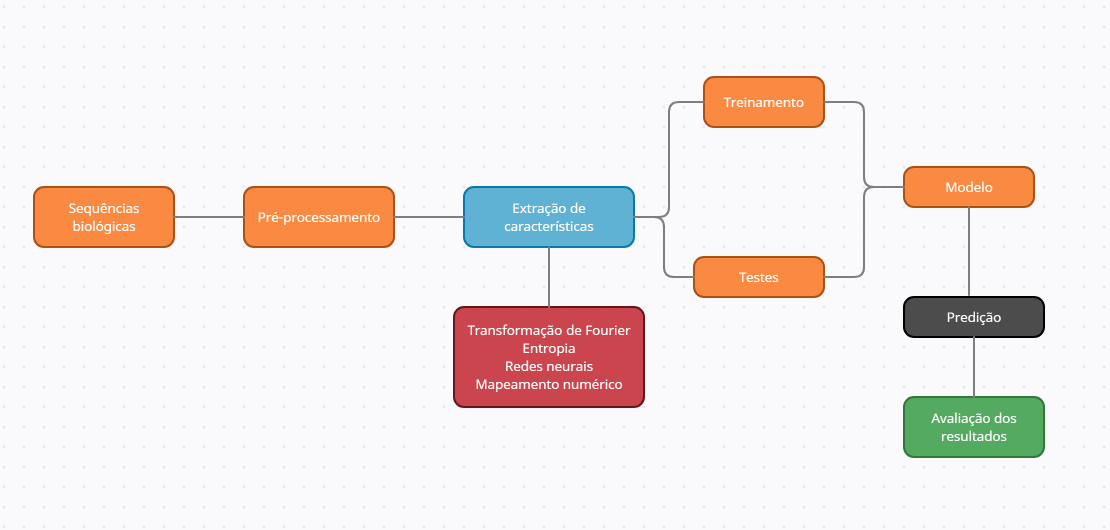
\includegraphics[width=1\textwidth]{images/fluxograma.png}
    \caption{Fluxograma de atividades criado pelo autor}
    \label{fig:workflow}
\end{figure}
  \chapter{Cronograma}

A tabela ~\ref{tab:cronograma} apresenta o período em que cada atividade deste trabalho será realizada.

\begin{table}[h!]
    \caption{Cronograma para a realização do TCC}
    \label{tab:cronograma}
    \begin{tabular}{p{6cm} c c c c c} % <-- Alignments: 1st column left, 2nd middle and 3rd right, with vertical lines in between
      \hline \\
      \textbf{Atividade} & \textbf{Setembro} & \textbf{Outubro} & \textbf{Novembro} & \textbf{Dezembro} & \textbf{Janeiro} \\
      \hline \\
      Coleta de dados brutos & X & - & - & - & - \\
      Pré-processamento dos dados coletados & X & - & - & - & - \\
      Implementação do algoritmo de classificação & - & X & - & - & - \\
      Treinamento e testes & - & X & - & - & - \\ 
      Avaliação do modelo & - & - & X & - & - \\
      Análise comparativa do método de \textit{machine learning} & - & - & - & X & - \\
      Escrita do TCC & X & X & X & X & X \\
      Revisão bibliográfica & X & X & X & X & X \\
      Defesa do TCC & - & - & - & - & X \\
      \hline \\
    \end{tabular}
\end{table}
  
  % References
  
  \begin{references}
    \bibliography{bib/references}
  \end{references}
  
  \end{document}
  